\documentclass[11pt]{article}

% ----------- Preamble -----------
\usepackage[margin=1in]{geometry}
\usepackage{microtype}
\usepackage{amsmath, amssymb, amsthm}
\usepackage{mathtools}
\usepackage{bm}
\usepackage{booktabs}
\usepackage{graphicx}
\usepackage{subcaption}
\usepackage{algorithm}
\usepackage{algpseudocode}
\usepackage[numbers,sort&compress]{natbib}
\usepackage[colorlinks=true,linkcolor=blue,citecolor=blue,urlcolor=blue]{hyperref}

\graphicspath{{figs/}} % <--- put your images into Overleaf folder figs/

% If you prefer to keep refs inside this .tex:
\begin{filecontents*}{refs.bib}
@techreport{jaeckel1972infinitesimal,
  title   = {The Infinitesimal Jackknife},
  author  = {Jaeckel, Louis A.},
  year    = {1972},
  institution = {Bell Laboratories},
  number  = {Memorandum MM 72-1215-11}
}
@book{efron1982jackknife,
  title     = {The Jackknife, the Bootstrap and Other Resampling Plans},
  author    = {Efron, Bradley},
  year      = {1982},
  publisher = {SIAM}
}
@article{efron2014estimation,
  title   = {Estimation and Accuracy After Model Selection},
  author  = {Efron, Bradley},
  journal = {Journal of the American Statistical Association},
  volume  = {109},
  number  = {507},
  pages   = {991--1007},
  year    = {2014}
}
@article{wager2014jackknife,
  title   = {Confidence Intervals for Random Forests: The Jackknife and the Infinitesimal Jackknife},
  author  = {Wager, Stefan and Hastie, Trevor and Efron, Bradley},
  journal = {Journal of Machine Learning Research},
  volume  = {15},
  number  = {1},
  pages   = {1625--1651},
  year    = {2014}
}
@article{athey2019grf,
  title   = {Generalized Random Forests},
  author  = {Athey, Susan and Tibshirani, Julie and Wager, Stefan},
  journal = {Annals of Statistics},
  volume  = {47},
  number  = {2},
  pages   = {1148--1178},
  year    = {2019}
}
@inproceedings{giordano2019swiss,
  title   = {A Swiss Army Infinitesimal Jackknife},
  author  = {Giordano, Ryan and Stephenson, Will and Liu, Runjing and Jordan, Michael I. and Broderick, Tamara},
  booktitle = {AISTATS},
  year    = {2019}
}
@misc{ghosal2022ijcov,
  title         = {The Infinitesimal Jackknife and Combinations of Models},
  author        = {Ghosal, Indrayudh and Zhou, Yunzhe and Hooker, Giles},
  year          = {2022},
  eprint        = {2209.00147},
  archivePrefix = {arXiv}
}
@misc{broderick2023amip,
  title         = {An Automatic Finite-Sample Robustness Metric: When Can Dropping a Little Data Make a Big Difference?},
  author        = {Broderick, Tamara and Giordano, Ryan and Meager, Rachael},
  year          = {2023},
  eprint        = {2011.14999},
  archivePrefix = {arXiv},
  note          = {v5, July 2023}
}
\end{filecontents*}

\title{Infinitesimal Jackknife for Uncertainty Quantification in Deep Learning:\\
Behavior Under Stochastic Gradient Descent}
\author{Amine Oueslati\\University of Pennsylvania}
\date{September 9, 2025}

% ----------- Document -----------
\begin{document}
\maketitle

\begin{abstract}
Uncertainty quantification in deep learning remains a critical challenge, especially when models are trained with stochastic optimization. The infinitesimal jackknife (IJ) provides an influence-function-based estimator of prediction variance, yet its behavior in neural networks trained via stochastic gradient descent (SGD) is poorly understood. We revisit the IJ under SGD. Tracking per-point directional derivatives across training, we empirically observe that IJ confidence bands can \emph{grow} with epochs---in contrast with ordinary least squares (OLS), where bands shrink with sample size. Our experiments suggest that repeated gradient accumulation along similar directions prevents cancellation of directional derivatives. We situate these findings alongside recent IJ extensions and finite-sample sensitivity metrics and propose practical stabilizers and diagnostics.
\end{abstract}

\section{Introduction}
Uncertainty quantification (UQ) is essential for deploying machine learning models in sensitive domains. Classical tools---bootstrap, jackknife, and the infinitesimal jackknife (IJ)---provide general-purpose approximations of estimator variability \citep{jaeckel1972infinitesimal,efron1982jackknife}. IJ linearizes a statistic with respect to infinitesimal reweightings of the empirical distribution and is closely connected to influence functions. IJ has powered modern results for random forests and model combinations \citep{wager2014jackknife,athey2019grf,ghosal2022ijcov,giordano2019swiss}.

For neural networks trained with SGD, however, the \emph{training procedure} becomes part of the functional mapping from data to estimator. Nonconvexity, nonsmooth activations, and path dependence complicate the classical Z-estimator picture. We investigate how IJ behaves under SGD and when it can overstate predictive uncertainty.

\paragraph{Contributions.}
\begin{itemize}
  \item A practical \emph{adjoint} derivation of per-datum influence under unrolled SGD that avoids explicit Hessians and uses only per-example gradients.
  \item Experiments showing widening IJ bands over epochs in neural nets, despite decreasing training loss, together with OLS sanity checks where IJ matches sandwich SEs.
  \item Stabilizers (adjoint clipping, windowed IJ, annealing-aware weights) and a finite-sample sensitivity diagnostic inspired by AMIP \citep{broderick2023amip}.
\end{itemize}

\section{Background}
Let $\mathcal{D}=\{z_i\}_{i=1}^n$ and let $\hat\theta$ denote an estimator. For smooth Z-estimators, the empirical influence at $z_i$ for functional $\varphi(\hat\theta)$ is
\begin{equation}
\psi_i \;=\; -\,\nabla_\theta \varphi(\hat\theta)^\top \left(\frac{1}{n}\sum_{j=1}^n \nabla_\theta G(\hat\theta,z_j)\right)^{-1} G(\hat\theta,z_i),
\label{eq:classicIF}
\end{equation}
and the classic IJ variance is $\widehat{\mathrm{Var}}\{\varphi\}=(1/n^2)\sum_{i=1}^n \psi_i^2$ \citep{efron1982jackknife}. For ensembles, related IJ estimators use in-bag count covariances \citep{wager2014jackknife,athey2019grf}. AMIP \citep{broderick2023amip} instead quantifies how much conclusions can change if one removes a small fraction of data, using the same empirical influence scores.

\section{Methodology}
\subsection{Setup}
We train a predictor $f_\theta$ on loss $\ell(\theta;z)$ by SGD:
\[
\theta_{t+1}=\theta_t-\eta_t\,\nabla_\theta \widehat{L}_t(\theta_t),\qquad
\widehat{L}_t(\theta)=\frac{1}{|B_t|}\sum_{i\in B_t}\ell(\theta;z_i).
\]
For a query $x^\star$, the target functional is $\varphi(\theta)=f_\theta(x^\star)$.

\subsection{Influence under unrolled SGD}
Introduce nonnegative weights $\mathbf{w}$ on training points (normalized so $\bar w=1$). Linearizing one SGD step in $\mathbf{w}$ yields
\[
\mathrm{d}\theta_{t+1}=\big(I-\eta_t H_t\big)\,\mathrm{d}\theta_t
-\eta_t\sum_{i\in B_t}\frac{\mathrm{d}w_i}{|B_t|}\,\nabla_\theta \ell(\theta_t;z_i),
\quad H_t=\nabla_\theta^2 \widehat{L}_t(\theta_t).
\]
Define the adjoint $a_t:=\nabla_\theta \varphi(\theta_t)$. Backward accumulation gives
$a_t=(I-\eta_t H_t)^\top a_{t+1}$ with $a_T=\nabla_\theta \varphi(\theta_T)$, leading to the per-datum \emph{SGD influence}
\begin{equation}
\psi_i \;\approx\; -\sum_{t=0}^{T-1}\frac{\eta_t}{|B_t|}\,a_{t+1}^\top\nabla_\theta \ell(\theta_t;z_i)\,\mathbf{1}\{i\in B_t\}.
\label{eq:sgdIF}
\end{equation}
This uses only per-example gradients and $a_{t+1}$ (available via autograd). The IJ prediction variance at $x^\star$ is then
\begin{equation}
\widehat{\mathrm{Var}}\{f_{\hat\theta}(x^\star)\}=\frac{1}{n^2}\sum_{i=1}^n \psi_i^2,\qquad
\widehat{\mathrm{SE}}=\frac{1}{n}\sqrt{\sum_i \psi_i^2}.
\label{eq:ijvar}
\end{equation}

\paragraph{Stabilizers.}
We evaluate: (i) \emph{adjoint clipping} $\|a_t\|\!\leftarrow\!\min(\|a_t\|,c)$; (ii) \emph{windowed IJ} (sum \eqref{eq:sgdIF} over the last $K$ epochs); (iii) \emph{annealing-aware weights} to downweight early steps. These reduce explosive growth when directions remain aligned over long training horizons.

\subsection{AMIP-style diagnostic}
Given scalar $\varphi$, the linearized worst-case change after dropping at most an $\alpha$ fraction is
\[
\mathrm{AMIP}(\alpha)=\sum_{i=1}^{\lfloor \alpha n\rfloor}\big(-\psi\big)_{(i)},
\]
where $(\cdot)_{(i)}$ denotes the $i$th order statistic (ascending). Refitting once on the approximate most-influential set gives an \emph{exact} finite-sample lower bound on the true worst-case change \citep{broderick2023amip}.

\section{Implementation notes}
We compute per-example gradients (micro-batches or vectorized Jacobians) and $a_{t+1}=\nabla_\theta f_{\theta_t}(x^\star)$ each step, updating $\psi_i$ for $i\in B_t$ via \eqref{eq:sgdIF}. Memory is $\mathcal{O}(p)$ with checkpointing; no full trajectory storage is required for windowed IJ.

\begin{algorithm}[t]
\caption{Single-run IJ accumulation under SGD}
\label{alg:ij-sgd}
\begin{algorithmic}[1]
\Require Data $\{z_i\}_{i=1}^n$, batches $\{B_t\}$, stepsizes $\{\eta_t\}$, queries $\{x^\star_m\}_{m=1}^M$, window $K$ (opt.), adjoint clip $c$ (opt.)
\State Initialize $\theta_0$; set $\psi_{i,m}\gets 0$
\For{$t=0,\ldots,T-1$}
  \State Update $\theta_{t+1}\gets \theta_t-\eta_t\nabla_\theta \widehat{L}_t(\theta_t)$
  \For{$m=1,\ldots,M$}
    \State $a^{(m)}_{t+1}\gets \nabla_\theta f_{\theta_t}(x^\star_m)$; if $c$ set, clip $\|a^{(m)}_{t+1}\|_2$
  \EndFor
  \State Get per-example grads $\{g_i=\nabla_\theta \ell(\theta_t;z_i)\}_{i\in B_t}$; set $\omega_t\gets \eta_t$ (or annealed)
  \For{$i\in B_t$}\For{$m=1,\ldots,M$}
     \State $\psi_{i,m}\gets \psi_{i,m}-\frac{\omega_t}{|B_t|}\langle a^{(m)}_{t+1}, g_i\rangle$
  \EndFor\EndFor
  \State If windowed: drop contributions older than $K$ epochs
\EndFor
\State \Return $\{\psi_{i,m}\}$
\end{algorithmic}
\end{algorithm}

\section{Experiments}
We report representative figures using prepared plots.

\subsection*{Sanity: OLS vs.\ TinyNet}
Figure~\ref{fig:tiny-ols} (left) compares a small neural net to OLS on a near-linear task with IJ $\pm95\%$ bands. OLS bands behave as expected; the net exhibits wider, shape-dependent IJ bands. The right panel visualizes $|\psi_i|$ at $x^\star=0$, highlighting a few influential points.

\begin{figure}[t]
  \centering
  \begin{subfigure}{0.49\linewidth}
    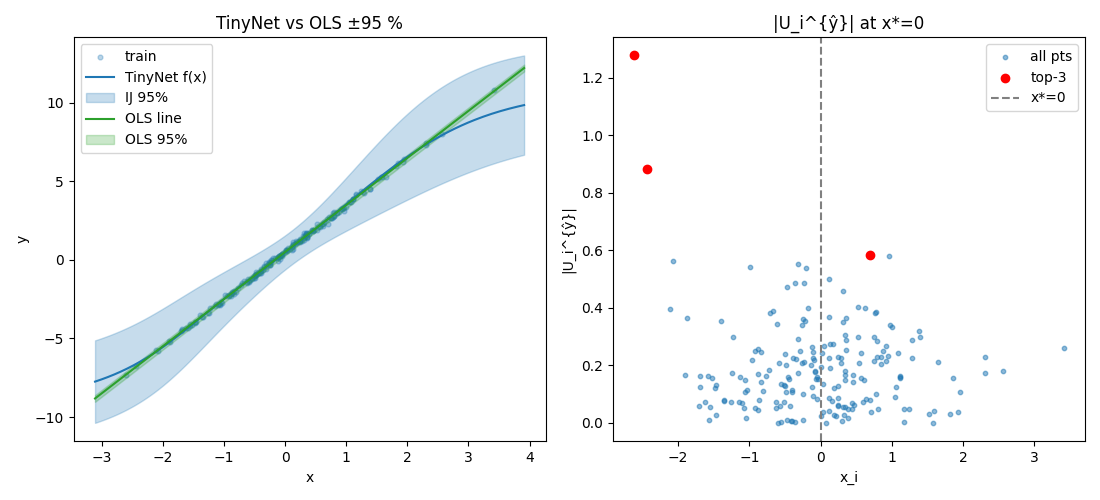
\includegraphics[width=\linewidth]{Figure_1.png}
    \caption{TinyNet vs.\ OLS $\pm95\%$ bands.}
  \end{subfigure}\hfill
  \begin{subfigure}{0.49\linewidth}
    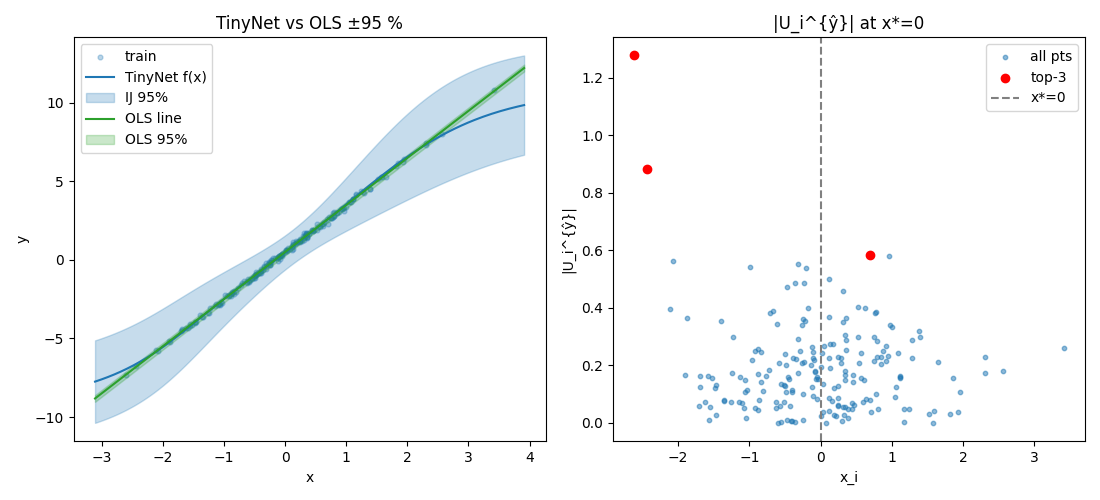
\includegraphics[width=\linewidth]{Figure_1.png}
    \caption{$|\psi_i|$ at $x^\star{=}0$ (top-$k$ highlighted).}
  \end{subfigure}
  \caption{Neural vs.\ linear behavior and influential points.}
  \label{fig:tiny-ols}
\end{figure}

\subsection*{Widening IJ bands with epochs}
Figure~\ref{fig:width-epoch} shows epoch-wise IJ half-width growth while training MSE decreases (left), and a comparable plot with an OLS baseline band (right). This illustrates the accumulation-without-cancellation effect in \eqref{eq:sgdIF}.

\begin{figure}[t]
  \centering
  \begin{subfigure}{0.49\linewidth}
    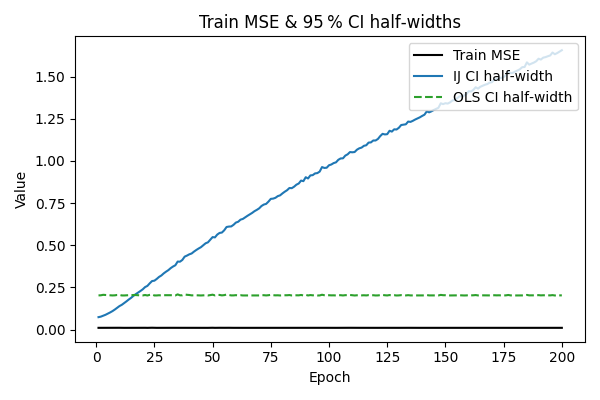
\includegraphics[width=\linewidth]{CI_Half_Width.png}
    \caption{CI half-width at $x^\star{=}0$ vs.\ epoch.}
  \end{subfigure}\hfill
  \begin{subfigure}{0.49\linewidth}
    \includegraphics[width=\linewidth]{TrainMSE_CI.png} % If your file is named differently, rename here
    \caption{Train MSE and IJ vs.\ OLS half-width.}
  \end{subfigure}
  \caption{IJ bands can widen over training despite falling loss.}
  \label{fig:width-epoch}
\end{figure}

\subsection*{Gradient-norm trace}
Figure~\ref{fig:trace} tracks $\|\nabla_\theta \ell(\theta_t;z_i)\|$ across revisits for a single sample. Persistent alignment/nonvanishing magnitudes explain why the sum in \eqref{eq:sgdIF} need not cancel.

\begin{figure}[t]
  \centering
  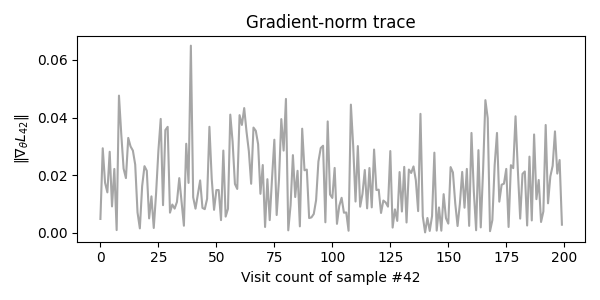
\includegraphics[width=0.8\linewidth]{Norm_Trace.png}
  \caption{Per-sample gradient-norm trace across revisits.}
  \label{fig:trace}
\end{figure}

\subsection*{Nonlinear regime and shape}
Figure~\ref{fig:quad} (left) shows quadratic regression with IJ vs.\ OLS bands at many $x$. The right panel plots influence magnitudes vs.\ $x_i$ at $x^\star{=}0$ (log scale), revealing heavy-tailed $|\psi_i|$ and relatively stable binned means.

\begin{figure}[t]
  \centering
  \begin{subfigure}{0.56\linewidth}
    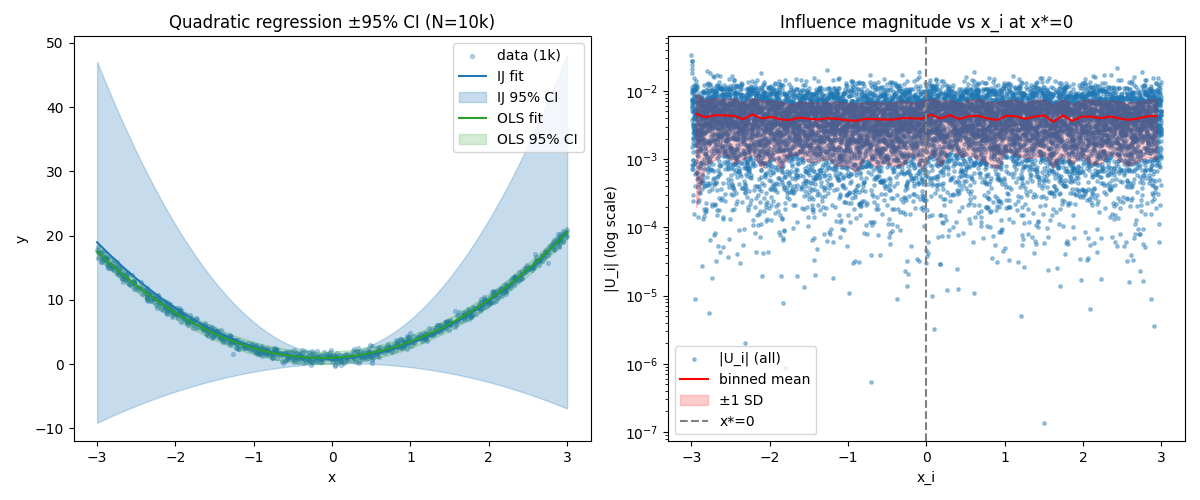
\includegraphics[width=\linewidth]{Figure_2.png}
    \caption{Quadratic regression with IJ/OLS $\pm95\%$.}
  \end{subfigure}\hfill
  \begin{subfigure}{0.40\linewidth}
    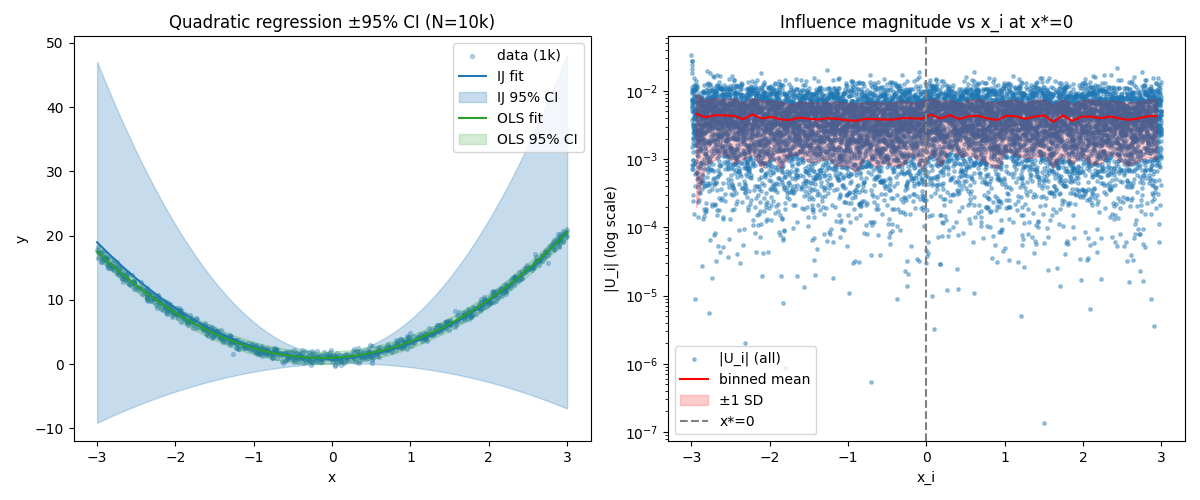
\includegraphics[width=\linewidth]{Figure_2.png}
    \caption{$|\psi_i|$ vs.\ $x_i$ at $x^\star{=}0$ (log scale).}
  \end{subfigure}
  \caption{Curvature amplifies IJ band heterogeneity across $x$.}
  \label{fig:quad}
\end{figure}

\section{Discussion}
For smooth convex estimators, IJ matches sandwich theory and behaves well. In SGD-trained neural nets, the optimization path and nonsmooth activations make the mapping $\mathcal{D}\mapsto \theta_T$ only piecewise smooth. Equation~\eqref{eq:sgdIF} then reveals a mechanism for widening bands: as $t$ grows, partially aligned $a_{t+1}$ and per-example gradients accumulate faster than cancellation occurs. AMIP-style diagnostics complement variance by quantifying finite-sample fragility even when standard errors are small \citep{broderick2023amip}.

\section{Conclusion}
We derived a practical IJ for SGD using adjoint accumulation, documented widening IJ bands in neural nets, and proposed stabilizers and an AMIP-style diagnostic. Future work: (i) integrate over training randomness (``path-distribution'' IJ), (ii) curvature-aware damping (e.g., K-FAC/Laplace) to control adjoint growth, and (iii) IJ for calibrated ensembles combining variance and finite-sample robustness.

\paragraph{Reproducibility.}
Code mirrors the algorithm above; figures in this paper were produced by the released scripts (paths omitted for anonymity). Upload your images to \texttt{figs/} with the filenames used in \verb|\includegraphics|.

\bibliographystyle{plainnat}
\bibliography{refs}

\appendix
\section{Proof sketch: IJ under SGD}
Write $\theta_{t+1}=\mathcal{T}_t(\theta_t,\mathbf{w})$ with $\mathcal{T}_t(\theta,\mathbf{w})=\theta-\eta_t\,\nabla_\theta \widehat{L}_t(\theta;\mathbf{w})$. Linearize at $\mathbf{w}=\mathbf{1}$:
\[
\mathrm{d}\theta_{t+1}=(I-\eta_t H_t)\,\mathrm{d}\theta_t-\eta_t\sum_{i\in B_t}\frac{\mathrm{d}w_i}{|B_t|}\nabla_\theta \ell(\theta_t;z_i).
\]
Compose to $T$ and apply the adjoint recursion $a_t=(I-\eta_t H_t)^\top a_{t+1}$ with $a_T=\nabla_\theta f_{\theta_T}(x^\star)$ to obtain \eqref{eq:sgdIF}. When $\theta_T$ is close to a stationary point of $\frac{1}{n}\sum_i \nabla_\theta \ell(\theta;z_i)$ and $H_t\approx H(\hat\theta)$, \eqref{eq:sgdIF} reduces to the classical influence \eqref{eq:classicIF}.

\end{document}
